%!TEX root = ../../thesis_master.tex

%%%%%%%%%%
\chapter{System Design}
\label{chap:system-design}
%%%%%%%%%%

In Chapter \ref{chap:theory-state-art} the theoretical basis of visual servo controllers and ROS systems were presented. Later, in Chapter \ref{chap:srs-sa}, the desired product was defined thanks to the \emph{Software Requirements Specification} and the \emph{Structured Analysis}. In this chapter, the system design adopted to achieve the above described product is presented.

%%%%%%%%%%
\section{Visual Servoing Task Breakdown}
\label{ref:task-breakdown}
%%%%%%%%%%

In order to complete its task, the system must use the five functions defined in Section \ref{sec:functional-requirements}, which can be divided in the following steps:

\begin{itemize}
	\item \textbf{Step 1}. Receive the desired target from the user.
	
	\item \textbf{Step 2}. Receive the desired pose with respect to the target from the user.
	
	\item \textbf{Step 3}. Compute the visual features from the desired pose to be used as desired features $\bm{s}^\ast$.
	
	\item \textbf{Step 4}. Detect the desired target.
	
	\item \textbf{Step 5}. Compute the visual features form the current pose to be used as current features $\bm{s}$.
	
	\item \textbf{Step 6}. Compute the feature difference to be used as control error and send to the user as feedback.
	
	\item \textbf{Step 7}. Compute the interaction matrix for the current features.
	
	\item \textbf{Step 8}. Compute the control linear velocity inputs in the camera frame.
	
	\item \textbf{Step 9}. Transform from the control linear velocity inputs from the camera frame to the robot frame.
	
	\item \textbf{Step 10}. Compute the target rotation around the $z\text{-axis}$.
	
	\item \textbf{Step 11}. Compute the control angular velocity input around the $z\text{-axis}$.
	
	\item \textbf{Step 12}. Send the velocity command to the low-level controller of the robot.
	
	\item \textbf{Step 13}. Stop when the control error has achieved a certain tolerance.
\end{itemize}
	
For \emph{Step 1} and \emph{Step 2}, a ROS action interface has been designed. The action interface implementation is explained in detail in the Section \ref{sec:ros_action}.	

The target used is an AprilTag (see Section \ref{sec:apriltag_markers}), a squared marker placed on the ground. Several markers can be present in the scene and the user must be able to select them. This feature is useful for a manipulator, since different targets may me necessary for its task. In a similar way, the user must be able of specifying the desired pose, so it can vary depending on the task to be conducted.

For \emph{Step 3}, the target's corners (3D coordinates in meters w.r.t. the object frame \{$O$\}) can be obtained, since the dimensions of the target are know. Using the desired pose, the corner coordinates are transformed to the camera frame \{$C$\} (3D coordinates in meters) and projected into the image plane (2D coordinates w.r.t. the camera frame \{$C$\} in pixels). With the pixel information, the desired image moment features are computed as described in Section \ref{sec:image-moments} so the $\bm{s}^\ast$ vector is obtained. Here the desired area of the target and the desired centroid coordinates are used as features.
 
Using the current image, the target is detected thanks to the detector described in Section \ref{sec:apriltag_markers}, so \emph{Step 4} is satisfied.
 
Once the desired target is detected its corner's coordinates are obtained already in the image plane (2D coordinates in pixels w.r.t. the camera frame \{$C$\}), so the current vector image moment features $\bm{s}$ can also be computed for \emph{Step 5}.

For \emph{Step 6}, the feature difference is computed as the subtraction $\bm{s} - \bm{s}^\ast$ and is given as feedback tanks to the action interface. The iteration matrices necessary for \emph{Step 7} were presented in Section \ref{sec:image-moments}.

The yaw rotation of the aerial robot is controlled by means of a proportional controller. The rotation of the target can be also computed (\emph{Step 10}) from the corner's coordinates as

\begin{equation}
 \theta_z = \arctan \left( \frac{tr_i - tl_i}{tr_j - tl_j} \right) 
\end{equation}
 
 Once the feature vectors have been computed, the control error can be obtained as $\bm{e} = \bm{s} - \bm{s}^\ast$ and together with $\theta_z$ are used to compute the control velocities (\emph{Step 8} and \emph{Step 11}) as described in Section \ref{sec:vs-algorithm-description}.
 
 The camera velocities are transformed to the robot frame \emph{Step 9} and used as input for the low level controller of the robot.
	
\begin{figure}[!htb]
		\caption{Interaction between the IBVS controller and the low-level controllers}
	\centering
	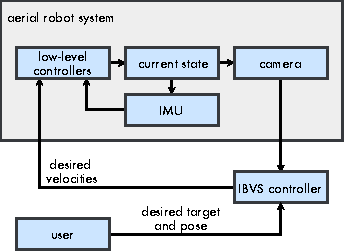
\includegraphics[width=0.5\textwidth]{content/chapter_04/images/context_diagram.pdf}
	\label{fig:low-level-ibvs}
\end{figure}

Putting all together, when the aerial robot simulation is started the action server for the visual servoing task is started. The robot can carry out any other mission, such as navigate to the target's position. Once the target is in the field of vision of the robot, the action client can be started. A desired pose with respect to the target is commanded and the client sends the goal to the server. The server receives the goal and creates a new visual servoing task for it. The desired features are computed taking into account the desired pose and the detector keeps tracking the AprilTag to get its corners and compute the current visual features. The visual feature difference is used as error for a proportional controller, which computes the required camera velocity to get an exponential decrease of the error. The computed velocities are transformed to into the robot frame and published to the low-level control velocity command. The low level control imposes this velocities on the robot while maintaining its stability. When a certain tolerance is reached, the robot is stopped and the client is notified about the final result and then shuts down. The robot is now able to start other mission and the visual servo controller available for a new request.

\newpage

The visual servoing control of the robot requires then three components:

\begin{itemize}
	\item The \emph{low-level} controllers of the aerial robot.
	
	\item The visual servoing controller implemented within the \emph{action interface}.
	
	\item The \emph{client} that uses the action interface to set a new visual servoing task.
\end{itemize}

\section{Visual Servoing Algorithm Description}
\label{sec:vs-algorithm-description}

In this section, an IBVS scheme for the control of the translation and yaw rotation kinematics \cite{bourquardez_2009} of an aerial robot is presented. The implementation details of this algorithm as a ROS system are given in Chapter \ref{chap:implementation}. 

As already mentioned in Section \ref{sec:vs-theory}, given a set of features $\bm{s}$, it is possible to relate the change of the features to the movement of the camera through the interaction matrix:

\begin{equation}
\dot{\bm{s}} = \bm{L_s} \bm{v}_c
\end{equation}

Generally speaking, the interaction term $\bm{L_s}$ depends nonlinearly on the state of the system and cannot be reconstructed exactly from the observed visual data. To cope with this situation the system can be linearized around an equilibrium position.

But it is possible to select a set of visual features that simplifies this matrices. In this case, the visual feature vector $\bm{s} = (x_n, y_n, a_n, \theta_z)$ is defined such that

\begin{equation*}
	a_n = Z^\ast \sqrt{\frac{a^\ast}{a}} \\
	x_n = a_n x_g \\
	y_n = a_n y_g \\
	\theta_z
\end{equation*}

Where $a$ is the area of the object in the image, $\left( x_g , y_g \right) $ are its centroid coordinates, $a^\ast$ the desired area, and $Z^\ast$ the desired depth between the camera and the target and $\theta_z$ the orientation of the object. The normalization of the initial quantities  is introduced for a better numerical stability in the computation of the interaction matrix \cite{tahri_2005}.

\pagebreak

 The convenience of the selected features lays on the decoupling for the control of the degrees of freedom. For a planar object which remains parallel to the image plane we have that:

\begin{itemize}
	\item The centroid's coordinates allow the control of the velocities in this plane.
	
	\item The area of the object is used to control the perpendicular distance between the object plane.
	
	\item The object orientation angle to compute the yaw angular velocity.
\end{itemize}

For an aerial robot where the camera is pointing downwards towards the target object, it is possible to assume that the velocities $\omega_x$ and $\omega_y$ stay small during all the trajectory. Thus, they do not contribute to the feature kinematics. So it can be written that

\begin{equation}
\dot{\bm{e}} = \dot{\bm{s}}
=
\begin{bmatrix}
\dot{x}_n\\ 
\dot{y}_n\\ 
\dot{a}_n\\ 
\dot{\theta}_z
\end{bmatrix}
=
\bm{L}_s
\begin{bmatrix}
v_x\\ 
v_y\\ 
v_z\\ 
\omega_x\\ 
\omega_y\\ 
\omega_z
\end{bmatrix}
\simeq
\bm{L}_s
\begin{bmatrix}
v_x\\ 
v_y\\ 
v_z\\ 
0\\
0\\
\omega_z
\end{bmatrix}
=
\bm{L}_s^{'}
\begin{bmatrix}
v_x\\ 
v_y\\ 
v_z\\ 
\omega_z
\end{bmatrix}
=
- \bm{I}_4 
\begin{bmatrix}
v_x\\ 
v_y\\ 
v_z\\ 
\omega_z
\end{bmatrix}
\end{equation}

As already mentioned in Section \ref{sec:vs-theory}, linear exponential stability is imposed on the error kinematics to ensure an exponential decoupled decrease for $\bm{e} = (\bm{s} - \bm{s}^\ast)$ (i.e. $\dot{\bm{e}} = - \lambda \bm{e}$, with $\lambda$ a positive gain). Now $\bm{e}$ can be used to compute the necessary camera velocities that reduce the error exponentially:

\begin{equation}
\begin{bmatrix}
v_x\\ 
v_y\\ 
v_z\\ 
\omega_z
\end{bmatrix}
=
- \lambda \left( \bm{L}_s^{'}\right)^+ \bm{e}
=
\lambda \bm{e}
\end{equation}

However, in order to get a better convergence, a PID controller is presented instead of a proportional controller. The objective of this PID controller is to compute the camera velocity so it minimizes the error computed as the difference between the current and the desired features:

\begin{equation}
\begin{bmatrix}
v_x\\ 
v_y\\ 
v_z\\ 
\omega_z
\end{bmatrix}
=
K_p \bm{e}(t) + K_i \int_0^t \bm{e}(\tau) d\tau + K_d \frac{d\bm{e}(t)}{dt}
\end{equation}

In order to transform the camera's velocities into the robot's velocities, in is necessary to multiply them by the velocity twist matrix:

\begin{equation}
\bm{V}_{EC}
= 
\begin{bmatrix}
1 & 1 & 1 & 0 & 0 & 1 \\
\end{bmatrix}
\begin{bmatrix}
\bm{R}_{EC} & \bm{t}_{EC} \times \bm{R}_{EC} \\ 
\bm{0}_{3 \times 3} & \bm{R}_{EC}
\end{bmatrix}
\end{equation}

Here, $\bm{R}_{EC}$ is the rotation matrix from \{C\} to \{E\} and $\bm{t}_{EC}$ the translation vector between the same frames.

The method presented in this section has some limitations, since it depends on the geometry of the target and considers only smooth and slow trajectories. Any aggressive maneuver, or a case in which the parallel target assumption is invalidated, makes the approximations taken fail.

In case that this algorithm was to be implemented into a fully-actuated aerial robot, it would be necessary to limit the degrees of freedom of the robot so it stays always parallel to the target. Thus, roll and pitch would not be considered. This restriction is no too heavy since the purpose of this work is acquiring a certain pose with respect to a target laying on the ground. 

In order to consider more aggressive maneuvers, the dynamics of the system must be taken into account. Several algorithms have been proposed for this purpose \cite{ozawa_2011} \cite{jabbari_dynamic_2012} \cite{ceren_image_2012}. To cope with the with the limitation of the target being parallel to the image plane, a virtual plane approach \cite{zheng_image-based_2017} can be introduced.

For aerial manipulators, it would be possible to use the above mentioned algorithm to place the robot near the target. Later, an additional visual servoing algorithm could be used to control the arm to conduct the manipulation task. However, in order to take advantage of a fully actuated mobile platform during the manipulation task, it would be specially interesting to use a weighted interaction matrix \cite{santamaria-navarro_uncalibrated_2017} to control not only the arm but also the mobile platform thanks to a partitioned control.